\documentclass[nobib]{tufte-handout}

%\\geometry{showframe}% for debugging purposes -- displays the margins

\newcommand{\bra}[1]{\left(#1\right)}
\usepackage{amssymb}
\usepackage{hyperref}
\usepackage[activate={true,nocompatibility},final,tracking=true,kerning=true,spacing=true,factor=1100,stretch=10,shrink=10]{microtype}
\usepackage{color}
\usepackage{steinmetz}
% Fixes captions and images being cut off
\usepackage{marginfix}
\usepackage{array}
\usepackage{tikz}
\usepackage{amsmath,amsthm}
\usetikzlibrary{shapes}
\usetikzlibrary{positioning}
\usepackage{listings}
\usepackage{caption}
\usepackage{circuitikz}
\DeclareCaptionFont{white}{\color{white}}
\DeclareCaptionFormat{listing}{\colorbox{gray}{\parbox{\textwidth}{#1#2#3}}}
\captionsetup[lstlisting]{format=listing,labelfont=white,textfont=white}

% Set up the images/graphics package
\usepackage{graphicx}
\setkeys{Gin}{width=\linewidth,totalheight=\textheight,keepaspectratio}
\graphicspath{{.}}

\title{Notes for ECE 20002 - Electrical Engineering Fundamentals II}
\author[Shubham Saluja Kumar Agarwal]{Shubham Saluja Kumar Agarwal}
\date{\today}  % if the \date{} command is left out, the current date will be used

% The following package makes prettier tables.  We're all about the bling!
\usepackage{booktabs}

% The units package provides nice, non-stacked fractions and better spacing
% for units.
\usepackage{units}

% The fancyvrb package lets us customize the formatting of verbatim
% environments.  We use a slightly smaller font.
\usepackage{fancyvrb}
\fvset{fontsize=\normalsize}

% Small sections of multiple columns
\usepackage{multicol}

% For finite state machines 
\usetikzlibrary{automata} % Import library for drawing automata
\usetikzlibrary{positioning} % ...positioning nodes
\usetikzlibrary{arrows} % ...customizing arrows
\tikzset{node distance=2.5cm, % Minimum distance between two nodes. Change if necessary.
    every state/.style={ % Sets the properties for each state
    semithick,
    fill=gray!10},
    initial text={}, % No label on start arrow
    double distance=2pt, % Adjust appearance of accept states
    every edge/.style={ % Sets the properties for each transition
    draw,
    ->,>=stealth', % Makes edges directed with bold arrowheads
    auto,
    semithick}}
\let\epsilon\varepsilon

% These commands are used to pretty-print LaTeX commands
\newcommand{\doccmd}[1]{\texttt{\textbackslash#1}}% command name -- adds backslash automatically
\newcommand{\docopt}[1]{\ensuremath{\langle}\textrm{\textit{#1}}\ensuremath{\rangle}}% optional command argument
\newcommand{\docarg}[1]{\textrm{\textit{#1}}}% (required) command argument
\newenvironment{docspec}{\begin{quote}\noindent}{\end{quote}}% command specification environment
\newcommand{\docenv}[1]{\textsf{#1}}% environment name
\newcommand{\docpkg}[1]{\texttt{#1}}% package name
\newcommand{\doccls}[1]{\texttt{#1}}% document class name
\newcommand{\docclsopt}[1]{\texttt{#1}}% document class option name

% Define a custom command for definitions and biconditional
\newcommand{\defn}[2]{\noindent\textbf{#1}:\ #2}
\let\biconditional\leftrightarrow

\begin{document}

\maketitle

\begin{abstract}
    These are lecture notes for spring 2024 ECE 20002 at Purdue. Modify, use, and distribute as you please.
\end{abstract}

\tableofcontents

\section{Course Introduction}

Continuation of Electrical Engineering Fundamentals I. The course addresses
mathematical and computational foundations of circuit analysis (differential
equations, Laplace Transform techniques) with a focus on application to linear
circuits having variable behavior as a function of frequency, with emphasis on
filtering. Variable frequency behavior is considered for applications of
electronic components through single-transistor and operational amplifiers. The
course ends with a consideration of how circuits behave and may be modeled for
analysis at high frequencies.\\~\\ Learning Objectives:
\begin{enumerate}
    \item Analyze 2nd order linear circuits with sources and/or passive elements
    \item Compute responses of linear circuits with and without initial conditions via
          one-sided Laplace transform techniques
    \item Compute responses to linear circuits using transfer function and convolution
          techniques
    \item Analyze and design transistor amplifiers at low, mid and high frequencies
\end{enumerate}

\pagebreak

\section{ECE 20001 Review}
Sinusoidal Signal (voltage and current) involve phasors, which bring complex
numbers to the forefront. When in Sinusoidal Steady State (SSS):\\
\begin{equation*}
    Z_R=R
\end{equation*}
\begin{equation*}
    Z_L=j\omega L
\end{equation*}
\begin{equation*}
    Z_C=\frac{1}{j\omega C}
\end{equation*}
This can in turn be represented as as the following function:\\
\begin{equation*}
    x(t)=K_0 cos(\omega t + \theta_0)
\end{equation*}
Which can be transformed into the following form:\\
\begin{align*}
    K_0 e^{j(\omega t + \theta_0)} & = K_0 e^{j \theta_0}                    \\
                                   & = K_0 (cos(\theta_0) + j sin(\theta_0)) \\
                                   & = K_0\phase{\theta_0}
\end{align*}
This can be represented as the following in the cartesian plane:\\
\begin{center}
    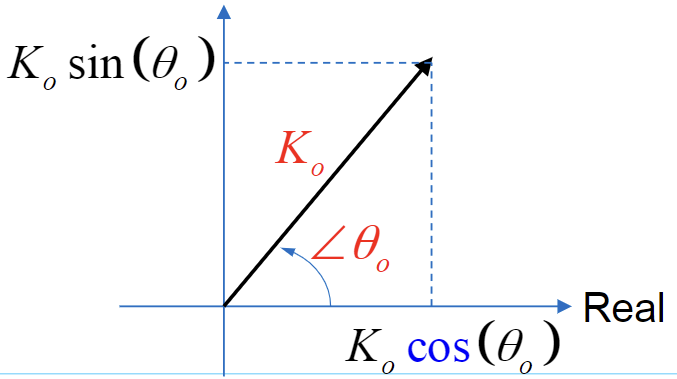
\includegraphics[width = 150px]{images/Screenshot 2024-01-08 155954.png}
\end{center}
Thus, these forms can be summed as following:\\
\begin{table}
    \centering
    \begin{tabular}{c|c}
        x(t)                                & $\mathbf{X}$ \\
        \hline
        $K cos(\omega t)$                   & K            \\
        $K sin(\omega t) = K cos(\omega t)$ & $-Kj$        \\
        $cos(\omega t) - sin(wt)$           & $1+j$        \\
        $a cos(\omega t) + b sin(\omega t)$ & $a-bj$
    \end{tabular}
\end{table}
This is especially useful for circuit analysis methods such as KCL and KVL.
The methods of conversion between polar and phasor are:\\
\begin{equation*}
    z=a+bj
\end{equation*}
\begin{equation*}
    z=\rho \phase{\theta}
\end{equation*}
\begin{equation*}
    \rho = |z| = \sqrt{a^2 + b^2}
\end{equation*}
\begin{equation*}
    \theta = \text{phase(}z\text{)}=tan^{-1}(\frac{b}{a})
\end{equation*}
These conversions and operations alongside KCL and KVL, can allow us to create a system of differential equations that will allow us to solve almost any circuit. However, we don't like ODEs, so we have developed methods to get around this.\\
We know that at SSS, the following equations are valid.
\begin{center}
    \begin{align*}
        V_R    & = RI_R                               \\
        V_L    & = j\omega LI_L                       \\
        V_C    & = \frac{1}{j \omega C}I_C            \\
        V_L(t) & = L\frac{di_L}{dt}        & \implies
        i_L(t) = i_L(0) + \frac{1}{L} \int v_L \,dt   \\
        i_C(t) & = C\frac{dV_C}{dt}        & \implies
        V_C(t) = V_C(0) + \frac{1}{C} \int i_C \,dt   \\
    \end{align*}
\end{center}
This can be used to solve most (to the knowledge of the student till this point) SSS circuits. Strategies have been developed to simplify these calculations. Some examples of this are current and voltage division, with the impedance $Z$ replacing the linear $R$. Strategies like these allow the resolution of circuits like these while avoiding higher order differential equations.\\
Example:
\begin{center}
    \begin{circuitikz}[american currents]
        \draw (0,0)
        to[I, l=$I$] (0,2)
        to [short, -*] (1,2)
        to [L, l=$L$] (1,0)
        to [short, -] (0,0);
        \draw (1,2)
        to [short, -*] (2,2)
        to [R, l=$R$] (2,0)
        to [short, *-*] (1,0);
        \draw (2,2)
        to [short, -] (2.5,2);
        \draw (2,0)
        to [short, -] (2.5,0);
    \end{circuitikz}
\end{center}
\begin{align*}
    I_R=\frac{Z_L}{Z_R+Z_L}*I=\frac{j \omega L}{R+j \omega L}*I \\
    I_L=\frac{Z_R}{Z_R+Z_L}*I=\frac{R}{R+j \omega L}*I
\end{align*}
If this circuit had an additional energy storing component, such as a capacitor
or an additional inductor, the complexity of current division does not increase
by a lot, but the differential equation would go from being a first-order differential
equation to a second-order differential equation. The complexity of this would be much
higher than that of the first-order differential equation, and would continue increasing
for each energy storing component that is added to the circuit.\\
Note: All of this is based on the assumption of \textbf{Sinusoidal Steady State}.
\\~\\
\begin{center}
    "We don't like differential equations." -Prof. Byunghoo Jung
\end{center}
\pagebreak
\section{Using Ordinary Differential Equations to solve RL and RC circuits}
This section will provide a brief explanation of nonhomogenous differential
equations and their applications to circuits (Completely ignoring the fact that
we in fact do not like them, as repeatedly stated in the previous section).
\subsection{Ordinary Differential Equations (ODE) Overview}
Differential equations rely a lot on two properties. The invariability of the
exponential function across derivatives, and the ability to express any
function in terms of the exponential function itself. That is,\\
\begin{equation*}
    e^t=\frac{d}{dt}e^t=\frac{d^2}{dt^2}e^t \cdots
\end{equation*}
Let us take the following differential equation as an example:
\begin{equation*}
    y(t)=6x(t)+3\frac{d}{dt}x(t)
\end{equation*}
Because of the beauty (invariability) of the exponential function, we assume $x_h(t)=Ae^{\lambda t}$, and try to solve the homogenous equation $0=6x(t)+3x'(t)$.
\begin{align*}
    0               & = 6x+3x'                                     \\
    0               & = 6Ae^{\lambda t} + 3A \lambda e^{\lambda t} \\
    0               & = 6+3\lambda                                 \\
    \lambda         & = -2                                         \\
    \implies x_h(t) & = e^{-2t}
\end{align*}
At this point, we will consider two different cases: $y(t) = 4e^{3t}$ and $y(t) = 3e^{-2t}$.
We will find the particular solution $x_p(t)$ for each of these cases, as they have different methods of resolution.
\begin{align*}
    4e^{3t}               & = 6x+3x'                                    \\
    \text{Assume } x_p(t) & = Be^{3t}                                   \\
    4e^{3t}               & = 6Be^{3t} + 9Be^{3t}                       \\
    4                     & = 15B                                       \\
    B                     & = \frac{15}{4}                              \\
    \implies x_p(t)       & = \frac{15}{4}e^{3t}                        \\
    \implies x(t)         & = x_h(t)+x_p(t)=Ae^{-2t}+\frac{15}{4}e^{3t}
\end{align*}
Let us assume $y(0) = 4$
\begin{align*}
    \implies 4    & = A + \frac{15}{4}                      \\
    \implies A    & = \frac{1}{4}                           \\
    \implies x(t) & = \frac{1}{4}e^{-2t}+\frac{15}{4}e^{3t}
\end{align*}
On the other hand, if $y(t) = 3e^{-2t}$, since $x_p(t)$ and $x_h(t)$ cannot have the same form, we will need to make a few changes:
\begin{align*}
    3e^{-2t}              & = 6x+3x'                              \\
    \text{Assume } x_p(t) & = Bte^{-2t}                           \\
    3e^{-2t}              & = 6Bte^{-2t} + 3Be^{-2t} - 6Bte^{-2t} \\
    \implies 3            & = 3B                                  \\
    \implies B            & =1                                    \\
    \implies x_p(t)       & = te^{-2t}
\end{align*}
Which can then be substituted into $x(t)$, allowing the differential equation to be fully solved by using the initial conditions.
\subsection{Using ODEs in circuits}
We will be solving the following two circuits (Note: you will never see
something like this with a current source instead, because it would be too
easy):
\begin{center}
    \begin{circuitikz}[american voltages]
        \draw (0,2)
        to[V, l=$V_{in}$] (0,0);
        \draw (0,2)
        to [R, l=$R$] (2,2)
        to [L, l=$L$] (2,0)
        to [short, -] (0,0);
    \end{circuitikz}
    \begin{circuitikz}[american voltages]
        \draw (0,2)
        to[V, l=$V_{in}$] (0,0);
        \draw (0,2)
        to [R, l=$R$] (2,2)
        to [C, l=$C$] (2,0)
        to [short, -] (0,0);
    \end{circuitikz}
\end{center}
In the inductor circuit, if $i_L(0)=0$, we know:
\begin{align*}
    v_L       & = L\frac{di_L(t)}{dt}                                  \\
    v_L(t)    & = v_{in}(t) + Ri_L(t)\text{ because of KVL}            \\
    v_{in}(t) & = L\frac{di_L(t)}{dt} + Ri_L(t)\text{ by substituting}
\end{align*}
By dividing the timeline into two sections, $(-\infty, 0) \text{ and } (0,\infty)$, and solving for the second one we can find our desired values for anytime in the future. However, for this to be a viable option, we need to solve for a continuous variable, which is $i$ for an inductor, and $v$ for a capacitor.\\
By solving this equation as shown previously, and looking for $i_L$, we will find that $\lambda = -\frac{R}{L}$ which is in fact the inverse of the time constant for an RL circuit.
Under the assumption of $V_{in}$ being a constant, the particular solution will in fact be $i_p(t)=\frac{V_{in}}{R}=i_L(\infty)$. This results in the familiar equation:
\begin{equation*}
    i_L(t) = i_L(\infty) + (i_L(t_0)-i_L(\infty))e^{-\frac{R}{L}(t-t_0)}
\end{equation*}
The same is done for the capacitor circuit, but this time looking for $v_C$, which ends up resulting in the once again familiar equation:
\begin{equation*}
    v_C(t) = v_C(\infty) + (v_C(t_0)-v_C(\infty))e^{-\frac{t-t_0}{RC}}
\end{equation*}
Note: energy storing components (L \& C) have memory but cannot consume power. R can consume power but has no memory.\\
Looking at this conceptually, the resistor is consuming energy at an exponential rate. This causes current, voltage, and all other signals to decay exponentially as well.\\
Since $P = I^2R = \frac{V^2}{R}$, it makes sense for the time constant to be $\tau = \frac{L}{R} = RC$, for each of them, as a larger capacitoror inductor would store more energy, and the proportionality of the R to the power and current or voltage respectively. That is, if R is larger, the power consumption is larger for an RL and smaller for an RC.\\
Note: the particular solution of the ODE is a scaled version of the input.\\
The homogenous solution will be the same for all inputs, and of the form $Ae^{\frac{-t}{\tau}}$.\\
The particular solution represents the behavior of the analyzed parameter when everything has settled down, or, at infinity.\\
We will now analyze the following circuits, which resemble the previous ones, but use voltage instead, and have teh components in parallel instead of series.
\begin{center}
    \begin{circuitikz}[american voltages, american currents]
        \draw (0,0)
        to[I, l=$I_{in}$] (0,2);
        \draw (0,2)
        to [short, -] (1,2)
        to [R, l^=$R$] (1,0)
        to [short, -] (2,0)
        to [L, l_=$L$] (2,2);
        \draw (0,0) to [short, -] (1,0);
        \draw (1,2) to [short, -] (2,2);
    \end{circuitikz}
    \begin{circuitikz}[american voltages, american currents]
        \draw (0,0)
        to[I, l=$I_{in}$] (0,2);
        \draw (0,2)
        to [short, -] (1,2)
        to [R, l^=$R$] (1,0)
        to [short, -] (2,0)
        to [C, l_=$C$] (2,2);
        \draw (0,0) to [short, -] (1,0);
        \draw (1,2) to [short, -] (2,2);
    \end{circuitikz}
\end{center}
The only solution we will analyze in this document, is the RC circuit, but the RL circuit can be similarly solved.
\begin{align*}
    i_{in}(t) &= C\frac{dv_C(t)}{dt}+\frac{1}{R}v_C(t)\\
    &\text{To solve this, we need to analyze the homogenous solution first,}\\ &\text{which is equivalent to there being no source in the circuit.}\\
    0 &= C\frac{dv_C(t)}{dt}+\frac{1}{R}v_C(t)\\
    0 &= RC\frac{dv_C(t)}{dt}+v_C(t)\\
    &\text{Assuming that $v_{C,h}(t) = Ae^{\lambda t}$, which results in:}\\
    0 &= RC \lambda^1 + \lambda^0 = RC \lambda +1\\
    \lambda &= -\frac{1}{RC} = -\frac{1}{\tau}\\
    \implies v_{C,h} &= Ae^{\frac{-t}{\tau}}
\end{align*}
All signals in a circuit of this form will also decay exponentially, just like in the previous cases.\\
Now we can solve for the particular solution of the ODE.\\
\begin{align*}
    i_{in}(t) &= C\frac{dv_C(t)}{dt}+\frac{1}{R}v_C(t)\\
    &\text{With a particular solution of the form $v_{C,p}=m$}\\
    k &= C\frac{d(m)}{dt}+\frac{1}{R}m=\frac{1}{R}m\\
    \implies m&=kR
\end{align*}
We can solve for inputs of constant, exponential, and sinusoidal inputs quite easily.
If $i_{in}(t) = 5e^{-3t}$, and thus $v_{C,p}=me^{-3t}$ and $v_C(0^-)=3$
\begin{align*}
    i_{in}(t)&= C\frac{dv_C}{dt}+\frac{1}{R}v_C\\
    5e^{-3t} &= -3Cme^{-3t}+\frac{1}{R}me^{-3t}\\
    5 &= \left(-3C+\frac{1}{R}\right)m\\
    \implies m &= \frac{5R}{-3RC+1}
\end{align*}
Substituting into the equation and using the initial value leads to the following final form:
\begin{align*}
    v_C(t) &= v_{C,h}(t) + v_{C,p}(t)\\
    &= Ae^{-\frac{t}{\tau}}+\frac{5R}{-3RC+1}e^{-3t}\\
    3&=A+\frac{5R}{-3RC+1}\\
    \implies A&=3-\frac{5R}{-3RC+1}
\end{align*}
and the final form will be:
\begin{equation*}
    v_C(t) = \left(3-\frac{5R}{-3RC+1}\right)e^{\frac{-t}{RC}}+\frac{5R}{-3RC+1}e^{-3t}
\end{equation*}
Similar solutions can be found for different inputs, and for RL circuits as well.
\end{document}